% для компиляции в lualatex!!
\documentclass[12pt, a4paper]{article}
\usepackage[english,russian]{babel}
\usepackage[warn]{mathtext}
%\usepackage[T2A]{fontenc}
%\usepackage[utf8]{inputenc}

\usepackage{xecyr} % Продукт Вашего покорного слуги ;)

\setmainfont{DejaVu Serif}

\usepackage{color}
\usepackage{amssymb,amsmath}
\usepackage{graphicx}
\usepackage{multicol}

\textheight=24cm           % высота текста
\textwidth=16cm            % ширина текста
\oddsidemargin=0pt         % отступ от левого края
\topmargin=-1.5cm          % отступ от верхнего края
\parindent=24pt            % абзацный отступ
\parskip=0pt               % интервал между абзацами
\tolerance=2000            % терпимость к "жидким" строкам
\flushbottom               % выравнивание высоты страниц
%\def\baselinestretch{1.5} % печать с большим интервалом

\title{Про размер маком возраста 1+.}
%\author{С.~А.~Назарова \thanks{e-mail:~sophia.nazarova@gmail.com}, Д.~А.~Аристов, А.~В.~Полоскин}
%\date{}

\begin{document}

\maketitle

\begin{description}
\item[Задача:] разделить моллюсков возраста 1+ и более старших.

\item[Материал:] В сборах 2012 года были отобраны все особи, размером менее 3 мм и у них измерена длина раковины и кольца зимней остановки роста (табл. \ref{tab:material_kolca}).

\begin{table}
\begin{tabular}{|p{0.5\textwidth}|*{2}{p{0.25\textwidth}|}} \hline
участок & количество проб & количество измеренных особей  \\ \hline
о. Горелый Лувеньгских шхер & 2 & 69 \\ \hline
Эстуарий р. Лувеньги & 3 & 49 \\ \hline
Литораль Западной Ряшковой салмы о. Ряшкова & 2 & 10 \\ \hline
\end{tabular}
\caption{Структура использованного материала}
\label{tab:material_kolca}
\end{table}

\item[Что получилось:] 
В данный размерный класс попали особи возрастом 1-3 года.
Их размеры различаются вот так (рис. \ref{ris:LengthAges}).
	\begin{figure}[h]
	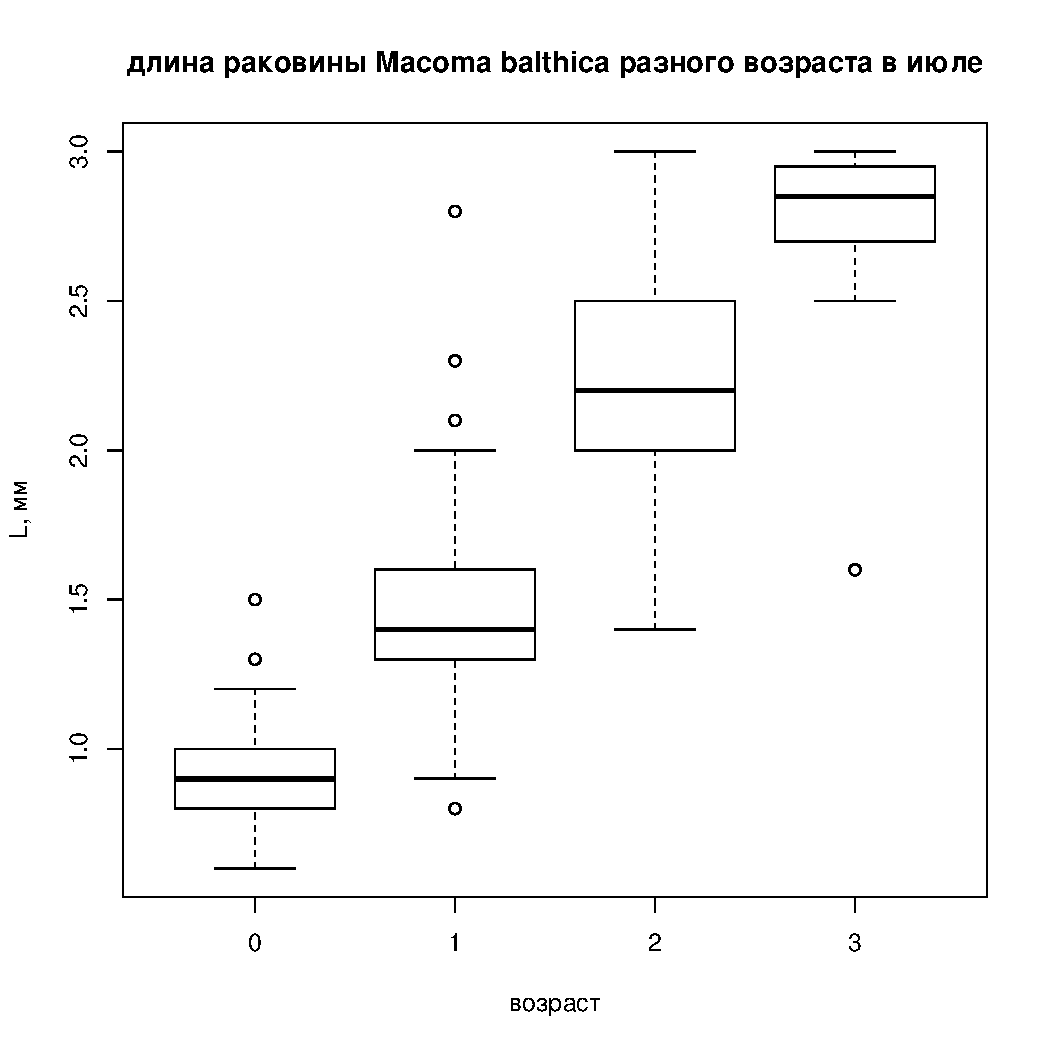
\includegraphics{/home/sonya/Dropbox/PhD_thesis/PhD_thesis/White_Sea/growth_young/boxplot_length_in_year.pdf}
	\caption{}
	\label{ris:LengthAges}
	\end{figure}


Нас интересует разделение особей 1+ и 2+ по длине. 
Размерная структура этих двух генераций выглядит следующим образом (рис. \ref{ris:hist_1_2}).
	\begin{figure}[h]
	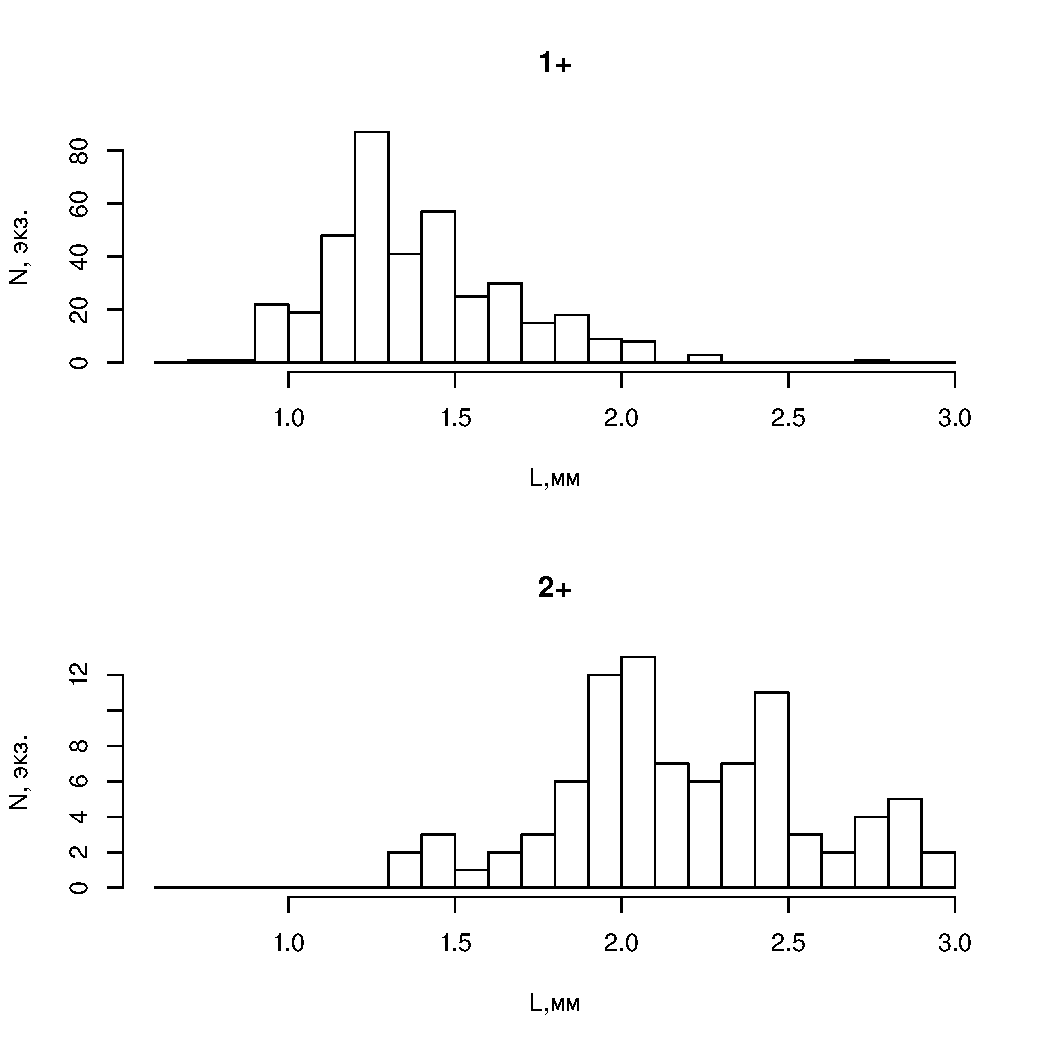
\includegraphics{/home/sonya/Dropbox/PhD_thesis/PhD_thesis/White_Sea/growth_young/hist_1year_2year.pdf}
	\caption{}
	\label{ris:hist_1_2}
	\end{figure}


Теперь вспоминаем, что участки у нас разные и смотрим различие длины особей возраста 1+ про участкам (разные горизонты Горелого тут идут вместе).
Результаты дисперсионного анализа  -- в таблице \ref{tab:anova1+} (это ANOVA, хотя, кажется, там для нее не все условия выполняются, но я смотрела и на Краскал-Уоллиcа, он тоже дает достоверные отличия, мне просто сейчас лень пересчитывать).

\begin{table}
\begin{tabular}{|*{6}{c|}} \hline
&Df&Sum Sq&Mean Sq&F value&Pr(>F) \\ \hline
area & 2 & 3,038 & 1,519 &21,291 & 5,196e-08 \\ \hline
Residuals & 73 & 5,2089 & 0,071 & & \\ \hline
\end{tabular}
\caption{Влияние участка на длину раковины моллюсков возрастом 1+}
\label{tab:anova1+}
\end{table}

Т.е. всячески влияет. 
И, по идее, теперь нам надо брать и таки мерить отдельно ракушек со всех участков, и всех считать отдельно.
На картинке это выглядит так  -- рис. \ref{ris:length1area}:
	\begin{figure}[h]
	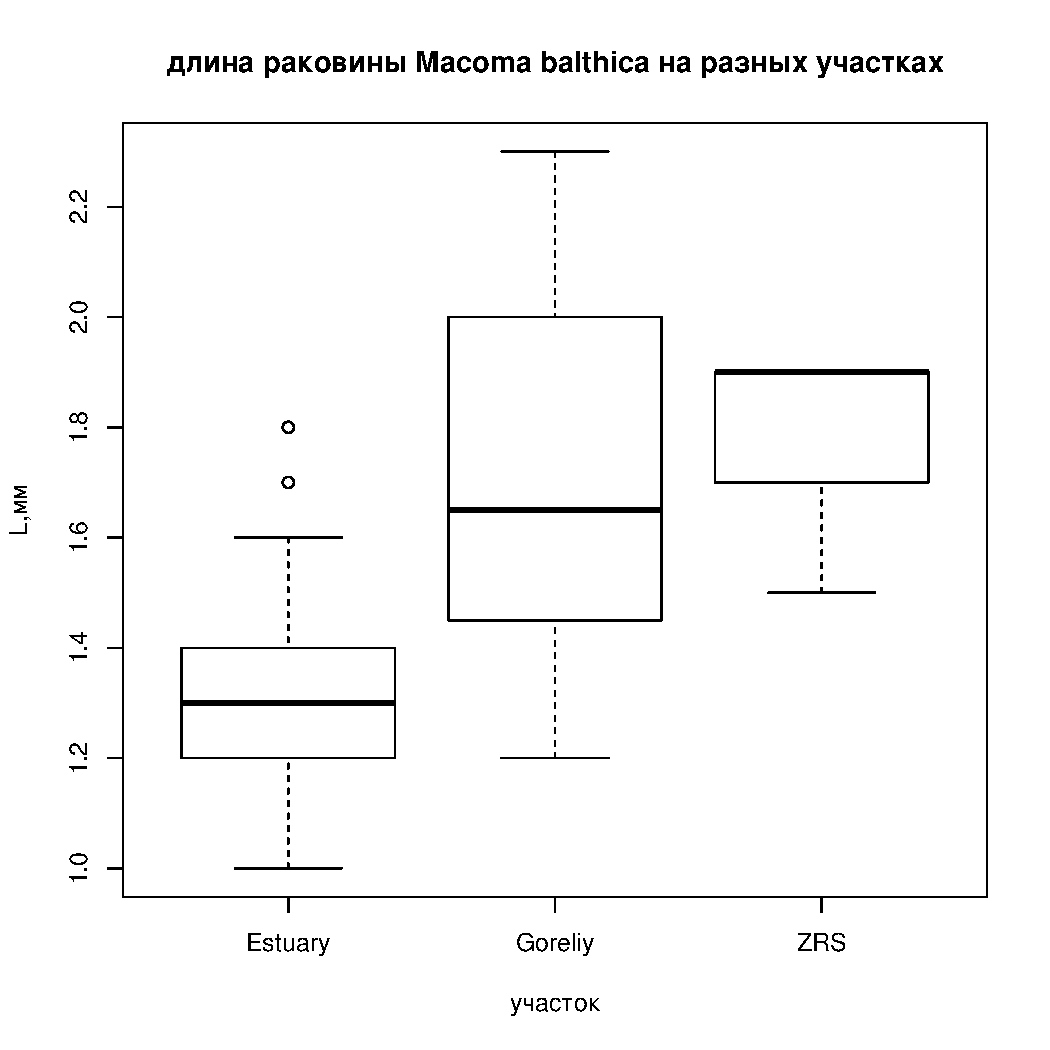
\includegraphics{/home/sonya/Dropbox/PhD_thesis/PhD_thesis/White_Sea/growth_young/boxplot_length_1+_area.pdf}
	\caption{}
	\label{ris:length1area}
	\end{figure}

\bigskip

Еще я смотрела на размер первого кольца (табл. \ref{tab:anova1k}). 

\begin{table}
\begin{tabular}{|*{6}{c|}} \hline
&Df&Sum Sq&Mean Sq&F value&Pr(>F) \\ \hline
area & 2 & 0,256 & 0,128 & 5,678 & 0,004 \\ \hline
age & 1 & 0,196 & 0,196 & 8,689 & 0,004 \\ \hline
area:age & 2 & 0,023 & 0,011 & 0,499 & 0,608 \\ \hline
Residuals & 121 & 2,731 &0,023 & & \\ \hline
\end{tabular}
\caption{Влияние участка и генерации на размер первого кольца остановки роста}
\label{tab:anova1k}
\end{table}

И тоже жизнерадостно все влияет. 
Хотя вот если посмотреть на картинку (рис. \ref{ris:k1_age_area}), то есть ощущение что разница меньше, чем в случае с июльским размером. 

	\begin{figure}[h]
	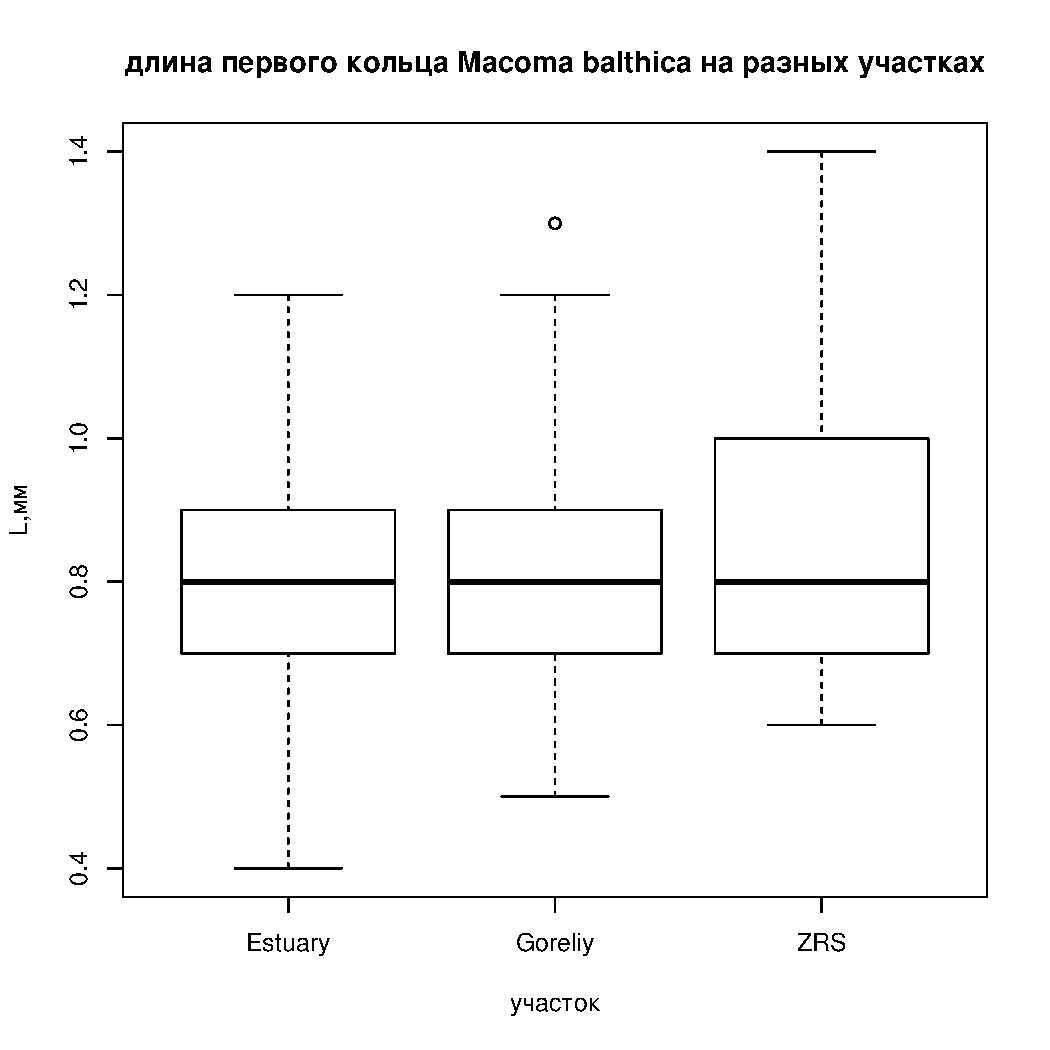
\includegraphics{/home/sonya/Dropbox/PhD_thesis/PhD_thesis/White_Sea/growth_young/boxplot_length_1kolco_area.pdf}
	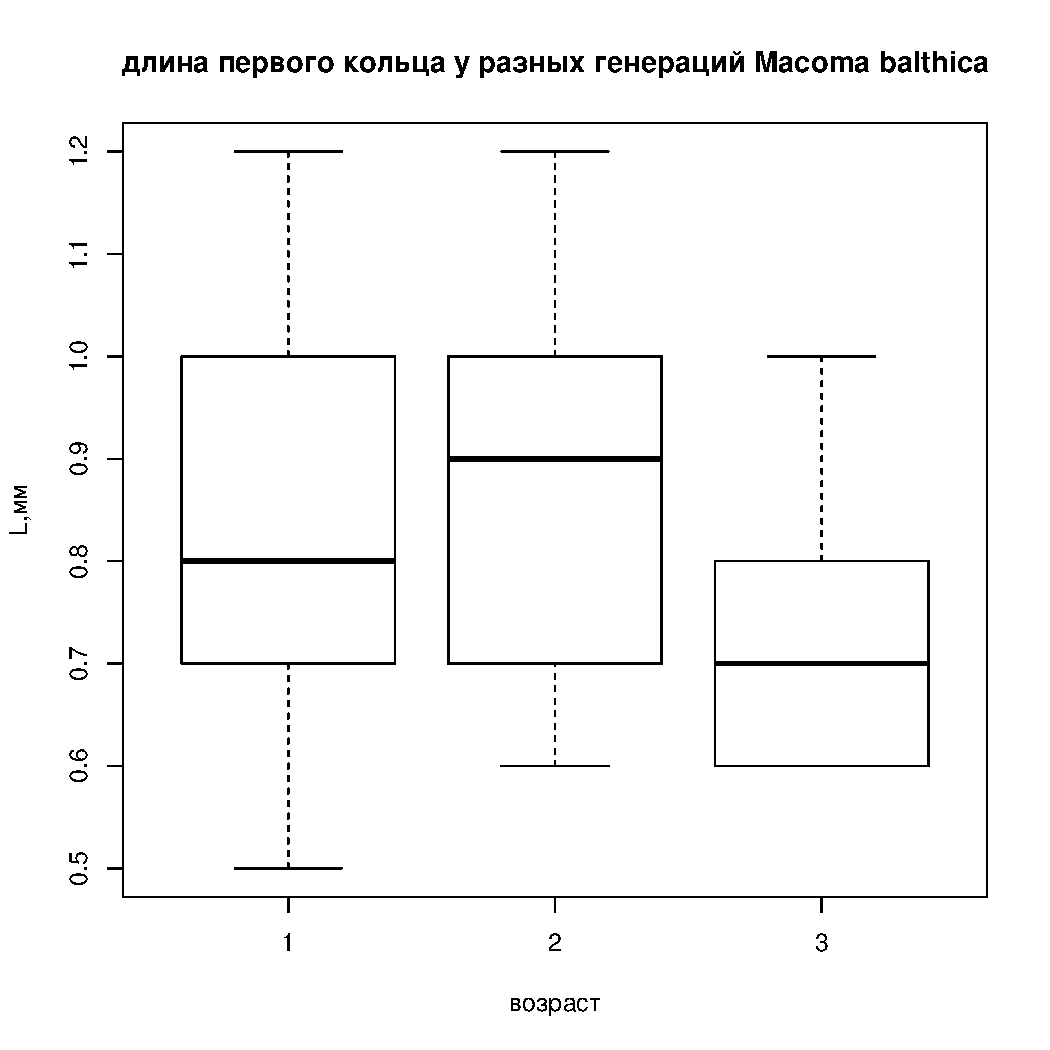
\includegraphics{/home/sonya/Dropbox/PhD_thesis/PhD_thesis/White_Sea/growth_young/boxplot_length_1kolco_age.pdf}
	\caption{}
	\label{ris:k1_age_area}
	\end{figure}

Но это уже и не имеет прямого отношения к тому, с чего все начиналось, просто любопытно.

Вопрос - что мы делаем с различием размера по участкам? 
И как делить?

Если не думать про участки, то распределения по размерам каждой генерации не нормальные. 
Если разделить, то несколько лучше (ЗРС не нормально распределено, но там маленькая выборка)

Если не думать про участки, то вот предлагаемые АВ 2 мм соотвествует 0,92~\% перцентилю для 1+ и 0,11~\% для 2+. То есть почти такие красивые 10\%

Конечно, правильнее (честнее) мерить все участки? Но у ДА нет фиксаций. Или вы сейчас на море померяете?


\end{description}
\end{document}
